\documentclass[10pt, conference, compsocconf,hyphens]{IEEEtran}
\usepackage{mathptmx}
\usepackage{amsmath}
%\usepackage{mathtools}
\usepackage{courier}
\usepackage[scaled=.92]{helvet}

\usepackage[pdfborder={0 0 0},bookmarks=false,breaklinks,draft]{hyperref}

\usepackage{graphicx}
\usepackage{color}
\usepackage{xspace}
\usepackage{listings}
\usepackage{booktabs,tabularx}
\usepackage[numbers,sort]{natbib}
\usepackage{ragged2e}
\usepackage{tikz}
\usepackage{dcolumn}
\usepackage{dsfont}
\usepackage{pdfpages}
\usepackage{listings}

\lstset{language=C,basicstyle=\ttfamily,xleftmargin=2em}

\iffalse % Change to \iffalse for submission
\usepackage{datetime}
\usepackage{fancyhdr}
\fancypagestyle{IEEEtitlepagestyle}{%
\fancyhead{}
\fancyfoot[L]{\textcolor{red}{\bfseries DRAFT}}
\fancyfoot[C]{\thepage}
\fancyfoot[R]{\textcolor{red}{\bfseries\currenttime\ \today}}
\renewcommand\headrulewidth{0pt}
\renewcommand\footrulewidth{0pt}}
\pagestyle{IEEEtitlepagestyle}
\fi
\usepackage{flushend}

\usepackage[binary-units]{siunitx}
\usepackage{subcaption}
\usepackage{multirow}
%\usepackage[title,header]{appendix}
\usepackage{lipsum}
\usepackage[absolute]{textpos}
\usepackage[T1]{fontenc}

\providecommand{\st}{\ensuremath{\mathrm{\ s.t.\ }}}

\providecommand{\bagmap}{\texttt{bagmap}}
\providecommand{\bagsum}{\texttt{bagsum}}
\providecommand{\bagsize}{\texttt{bagsize}}
\providecommand{\bagsplit}{\texttt{bagsplit}}

\providecommand{\lone}{\ensuremath{\ell{}_1}}

\hyphenation{white-list}

% taken from hs's mary.tex, and tracing back to knuth.
\def\dash---{\kern.16667em---\penalty\exhyphenpenalty\hskip.16667em\relax}

% C++ macro from john mitchell
\def\CC{C\raise.22ex\hbox{{\footnotesize +}}\raise.22ex\hbox{\footnotesize +}\xspace}

% Make URLs linebreak better (hat-tip alexras)
  % A sequence of BigBreaks will be treated as one break, so it will only be able to break after ://
  \renewcommand{\UrlBigBreaks}{\do\:\do\/}
  % (Less aggressive) Treat both / and - as breakable characters (don't know why this does something different than hyphens in the package declaration, but it does)
  \renewcommand{\UrlBreaks}{\do\/\do\-}
  % (More aggressive) Any letter and / are treated as breakable characters
  \renewcommand{\UrlBreaks}{\do\/\do\a\do\b\do\c\do\d\do\e\do\f\do\g\do\h\do\i\do\j\do\k\do\l\do\m\do\n\do\o\do\p\do\q\do\r\do\s\do\t\do\u\do\v\do\w\do\x\do\y\do\z\do\A\do\B\do\C\do\D\do\E\do\F\do\G\do\H\do\I\do\J\do\K\do\L\do\M\do\N\do\O\do\P\do\Q\do\R\do\S\do\T\do\U\do\V\do\W\do\X\do\Y\do\Z}

\lstdefinelanguage{JavaScript}{
  morekeywords={typeof, new, true, false, catch, function, return, null, catch, switch, var, if, in, while, do, else, case, break},
  morecomment=[s]{/*}{*/},
  morecomment=[l]//,
  morestring=[b]'',
  morestring=[b]'
}

\lstdefinelanguage{HTML5}{
        language=html,
        sensitive=true,
        alsoletter={<>=-},
        otherkeywords={
        % HTML tags
        <feConvolveMatrix, />
        },
        ndkeywords={
        % General
        =,
        % HTML attributes
        charset=, id=, width=, height=, in=, order=, edgeMode=, kernelMatrix=, preserveAlpha=,
        % CSS properties
        border:, transform:, -moz-transform:, transition-duration:, transition-property:, transition-timing-function:,
        },
        morecomment=[s]{<!--}{-->},
        tag=[s]
}

\lstset{%
    % Code
    language=HTML5,
    alsolanguage=JavaScript,
    showstringspaces=false,
    extendedchars=true,
    breaklines=true
 }

\providecommand{\setjmp}{\texttt{setjmp}}
\providecommand{\longjmp}{\texttt{longjmp}}

% Alter some LaTeX defaults for better treatment of figures:
    % See p.105 of "TeX Unbound" for suggested values.
    % See pp. 199-200 of Lamport's "LaTeX" book for details.
    %   General parameters, for ALL pages:
    \renewcommand{\topfraction}{0.99}    % max fraction of floats at top
    \renewcommand{\bottomfraction}{0.8} % max fraction of floats at bottom
    %   Parameters for TEXT pages (not float pages):
    \setcounter{topnumber}{2}
    \setcounter{bottomnumber}{4}
    \setcounter{totalnumber}{6}         % 2 may work better
    \setcounter{dbltopnumber}{6}        % for 2-column pages
    \renewcommand{\dbltopfraction}{0.99} % fit big float above 2-col. text
    \renewcommand{\textfraction}{0.07}  % allow minimal text w. figs
    %   Parameters for FLOAT pages (not text pages):
    \renewcommand{\floatpagefraction}{0.7}  % require fuller float pages
    % N.B.: floatpagefraction MUST be less than topfraction !!
    \renewcommand{\dblfloatpagefraction}{0.7} % require fuller float pages


\setlength{\TPHorizModule}{30mm}
\setlength{\TPVertModule}{\TPHorizModule}
\textblockorigin{10mm}{10mm}

\newcolumntype{C}[1]{>{\centering\let\newline\\\arraybackslash\hspace{0pt}}m{#1}}

% get rid of that stupid box on the first page.
\makeatletter
\def\@copyrightspace{}
\makeatother

% Support cool highlighting boxes in lstlisting (from
% http://tex.stackexchange.com/questions/15237/highlight-text-in-code-listing-while-also-keeping-syntax-highlighting)
\makeatletter
\newenvironment{btHighlight}[1][]
{\begingroup\tikzset{bt@Highlight@par/.style={#1}}\begin{lrbox}{\@tempboxa}}
{\end{lrbox}\bt@HL@box[bt@Highlight@par]{\@tempboxa}\endgroup}

\newcommand\todo[1]{\textcolor{red}{TODO:#1}}

\newcommand\btHL[1][]{%
  \begin{btHighlight}[#1]\bgroup\aftergroup\bt@HL@endenv%
}
\def\bt@HL@endenv{%
  \end{btHighlight}%
  \egroup
}
\newcommand{\bt@HL@box}[2][]{%
  \tikz[#1]{%
    \pgfpathrectangle{\pgfpoint{1pt}{0pt}}{\pgfpoint{\wd #2}{\ht #2}}%
    \pgfusepath{use as bounding box}%
    \node[anchor=base west, fill=orange!30,outer sep=0pt,inner xsep=1pt, inner ysep=0pt, rounded corners=3pt, minimum height=\ht\strutbox+1pt,#1]{\raisebox{1pt}{\strut}\strut\usebox{#2}};
  }%
}
\lstdefinestyle{Chighlight}{
    language={C},basicstyle=\ttfamily,
    moredelim=**[is][\btHL]{`}{`},
    moredelim=**[is][{\btHL[fill=green!30,draw=red,dashed,thin]}]{@}{@},
}
\makeatother


% support aligning a table column on .
\newcolumntype{d}[1]{D{.}{.}{#1} }

\def\sharedaffiliation{
\end{tabular}
\begin{tabular}{c}}
\begin{document}


\title{802.11ac performance in reality}

\author{
\IEEEauthorblockN{David Kohlbrenner, Jake Maskiewicz, Sean Hamilton}
\IEEEauthorblockA{
University of California, San Diego\\
}
}


\clubpenalty=10000
\widowpenalty=10000

\maketitle

%\section{Schedule}

%A schedule, specifying concretely what you intend to have accomplished by each
%of the two milestones below as well as for the final report/presentation. It is
%perfectly acceptable if the final deliverable is not a completion of the
%project---which, if successful, some members of the group may wish to continue
%after the term ends---but it does need to be something that can be clearly
%demonstrated/evaluated/graded.

Our original goals have (as we discussed) had to change. This will outline (briefly) what we hope to have done for the presentation and talk.
Obviously its less than we would have preferred, but we have less time than we would've liked to run these experiments.

\begin{enumerate}
\item Test throughput as a function of distance for the new 80MHz bandwidth and compare to the 20/40Mhz bandwidth options that were defined in 802.11g and n standard
\item Provide a theoretical analysis of throughput for 160Mz channel bandwidth as a function of distance (Our equipment doesn't support 160MHz)
\item Test throughput for the newer modulation 256QAM modulation scheme and the two accompanying FEC codings (MCS 8 and 9)
\item Test and analyze the throughput and parallelism of MU-MIMO that is supported in 802.11ac
\end{enumerate}

\section{background}

Today we see the now ubiquitous WiFi networks in almost every setting where computers are used from home and businesses to public WiFi hotspots. This trend has grown over the years as mobile devices such as smart phones require high-speed network access and laptops are frequently reducing their port count eliminating wired network options.

The IEEE 802.11 standard for wireless Ethernet has evolved over the years to keep pace with these ever increasing demand for higher throughput wireless network connectivity.

\subsection{Previous Standards}

There were four widely used versions of 802.11 before ac; b, g, a, and n. The first widely used version, b, was introduced in September 1999 and is still seen in use today in many lower-end devices. This version operated in the 2.4GHz spectrum and made use of eleven 22MHz channels in the US and fourteen in some countries. The b standard uses Direct-Sequence Spread Spectrum (DSSS) as the only modulation scheme dropping the Frequency-Hopping Spread Spectrum (FHSS) that was used in legacy versions of 802.11 prior to the release of b. At the same time that b was released the a standard was also released placing DSSS with Orthogonal Frequency Division Multiplexing (OFMD) as the modulation scheme and changing from 22MHz to 20MHz bandwidth channels in the 5GHz spectrum. This allowed for data rates of up to 54Mbps. The next standard, g, brought the modulation schemes and 20MHz channel bandwidth over from the a standard to the 2.4GHz spectrum while maintaining backwards compatibility by support modulation and channel bandwidths of b. 

The next standard, n, which ac builds upon and simplifies further, aims to consolidate technologies used on both 2.4GHz and 5GHz while obsoleting outdated parts of the standard while introducing a few new capabilities that worked on both spectrums to increase throughput and efficiency. The n standard removes backwards compatibility from a,b and g standards although the reality is most hardware still implements these standards for maximum compatibility. Noticeably missing is DSSS The standard adds three main capabilities to the 802.11 standard; Multi-Input Multi-Output (MIMO) and 40 MHz bandwidth channels to the phy layer and frame aggregation to the MAC layer. 

\begin{table*}[b]
\caption{Summary of IEEE 802.11 Capabilities}
\begin{center}
\begin{tabular}{c | c | c | c | p{1.3cm} | c}
\textbf{revision} & \textbf{release data} & \textbf{spectrum (GHz)} & \textbf{bandwidth (MHz)} & \textbf{modulation} & \textbf{spatial streams} \\
\hline\hline
a & 9/1999 & 5 & 20 & OFDM & N/A \\ \hline
b & 9/1999 & 2.4 & 22 & CCK\newline DSSS & N/A \\ \hline
g & 6/2003 & 2.4 & 20 & CCK\newline OFDM\newline DSSS & N/A \\ \hline
n & 10/2009 & 2.4/5 & 20/40 & OFDM & 4 \\ \hline
ac & 12/2013 & 5 & 20/40/80/160 & OFDM & 8 \\ \hline
\end{tabular}
\end{center}
\label{table:80211caps}
\end{table*}

\subsection{IEEE 802.11ac}

\subsubsection{Changes to Previous Standards}


\subsubsection{802.11ac Specific Features}



\subsection{Future of Wireless Networks}



\section{Methodology}
\label{sec:methodology}

We tested various devices against our 802.11ac WAP in both clear and RF-noisy
environments. We originally planned to measure the differences between several
different MCSs, on both 80MHz and 40MHz, and the effects of MU-MIMO and
beamforming on a connection. Unfortunately, due to hardware limitations, we were
only able to test 80 MHz vs 40MHz, and monitor some beamforming and MCS activity
without influencing or selecting it.

\subsection{Devices}

\paragraph{RF Test Equipment}

We used a spectrum analyzer that is capable of monitoring 2.4GHz and 5GHz WiFi
signals allowing us to see all RF traffic in the spectrums beyond just WiFi.
We used it to observe active networks and to confirm that our clear testing
location had minimal to no RF noise.

\paragraph{Wireless APs}

Our WAP is the latest hardware model of the Linksys WRT1900AC 802.11ac,
with a 1.2 GHz dual core ARM processor and 256MB of DDR3 RAM. We originally
installed OpenWRT Chaos Calmer (Dev Branch) on the AP, because we believed it
would give us complete configuration control and insight into what the AP is
doing. Unfortunately, after many tests, we determined that bugs or
inefficiencies in the OpenWRT firmware were causing issues with our throughput
numbers, and we restored the original Linksys stock firmware to the device.
After doing so, our results returned to the expected levels for throughput.

\paragraph{Clients}

We used a number of devices as 802.11ac clients, including an 2013 Apple
Macbook Pro 15" Retina, a Microsoft Surface Pro 3, and a
Lenovo T420s (running Debian Jessie on a mainline 3.19 Linux kernel)
with a Intel 7260 series PCIe 802.11ac capable wifi card installed.

We also purchased an ASUS USB-AC56 801.11ac dongle so that we could
utilize any other non-ac host as an ac host for testing. However after
a small number of tests, the ASUS dongle began to experience
intermittent USB disconnections. Paired with its poor driver
performance, we did not continue testing with it.

\subsection{Testing}

\paragraph{Setup}
To run our tests, we connected one computer via ethernet cable to the AP, and
then connected the device we were testing over 802.11ac wireless. We would then
run an iperf version 2 server on the wireless client, and
an iperf client on the hardwired device. This way the flow of data over wifi
would be from the router to the wireless client. For a majority of our tests, we
did four transfers of 250MB, though for some tests, we did one transfer lasting
100 seconds. For a majority of tests, we captured packets either on the device
doing the transfer itself, or on a nearby device using monitor mode. This way
we could get high level throughput information from iperf, and then examine the
packet captures afterwards to help understand and explain our results.

\paragraph{Locations}
We wanted to perform our tests in both RF-clear and RF-noisy
environments. For the noisy environment, we used our offices in the
CSE building, which are surrounding by 802.11b/g/n/ac APs and
devices. For the clear environment, we performed initial promising
tests in the basement level of the Hopkins parking structure, however
we were concerned that the low concrete beams in the ceiling could be
inadvertently effecting our results. We then moved out to the parking
lot behind the Torrey Pines glider port. Here we had a wide open space
with no RF-interference according to our spectrum analyzer. Note that
our RF scan preceeded our actual testing by a little over a week, so
it is possible that at the time of testing there was a source of noise
in the 5GHz range.


\paragraph{Indoor}
In the office, we set the WAP at a fixed point, and then measured out 5, 10 and
15ft increments from the device for initial tests. We then moved our clients out
into the hallway, so the signal had to travel approximately 19 feet and through
a single wall. Then we measured from the kitchen, so the signal had to travel
through two walls for a total distance traveled of approximately 23 feet, and
then on the other side of the building, approximately 51 feet away, so that the
signal had to travel through several walls and devices. We tested each of our
devices with the WAP set to both 80MHz and 40MHz.  However, we were unable to
force the WAP or any of the clients to stick to a single MCS, and we were unable
to disable or influence beamforming on any of the clients.

\paragraph{Clear}
Out at the glider port, we measured out several different distances from the
router and ran tests from there. Because of the size of the parking lot, we were
able to run tests much further away from the router here than in the office.

\paragraph{Measurements}
We tested each of our devices with the WAP set to both 80MHz and 40MHz.
However, we were unable to force the WAP or any of the clients to stick to a
single MCS, and we were unable to disable or influence beamforming on any of the
clients. Because of this, we were only able to observe the effects of
beamforming or different MCSs as they normally occurred. We also captured throughput
from the iperf utility to measure TCP performance as a function of distance for the measurements
above as a function of distance.

\subsection{MU-MIMO Testing}

We also originally intended to measure the effect of MU-MIMO on
throughput and packet drops, however we ran into some
complications. Of the three chipset drivers that support MU-MIMO, none
have any client products that are currently on the market. So although
our WAP supported MU-MIMO, no clients exist that support MU-MIMO.

Despite this, we set up what we believe is a strong experimental design to test
MU-MIMO and confirm that it is occurring through monitoring the clients. The
setup is as follows:

There are two wireless connected laptops running iperf servers, as in the
previously described setup. These two clients should be placed on opposite sides
or orthogonal to the router at some fixed distance. Near these laptops, two more
laptops with their wireless cards placed in monitor mode will log all the
packets they receive.

Then, connected via ethernet to the AP will be two iperf clients, so that data
flow travels from the router to the wireless clients. A third device will be
connected to the AP via ethernet which broadcasts an increasing index and a
64-bit timestamp every 100 milliseconds. This way, we can correlate runs of
packets between broadcasts with matching indexes and monitor clock skew.

We believe that, given proper MU-MIMO hardward, this testing setup would be
capable of confirming that MU-MIMO is indeed happening, and allowing us to
reason about its effects on the network.

\section{Results}
\todo{results}
\begin{figure}[!h]
\centering
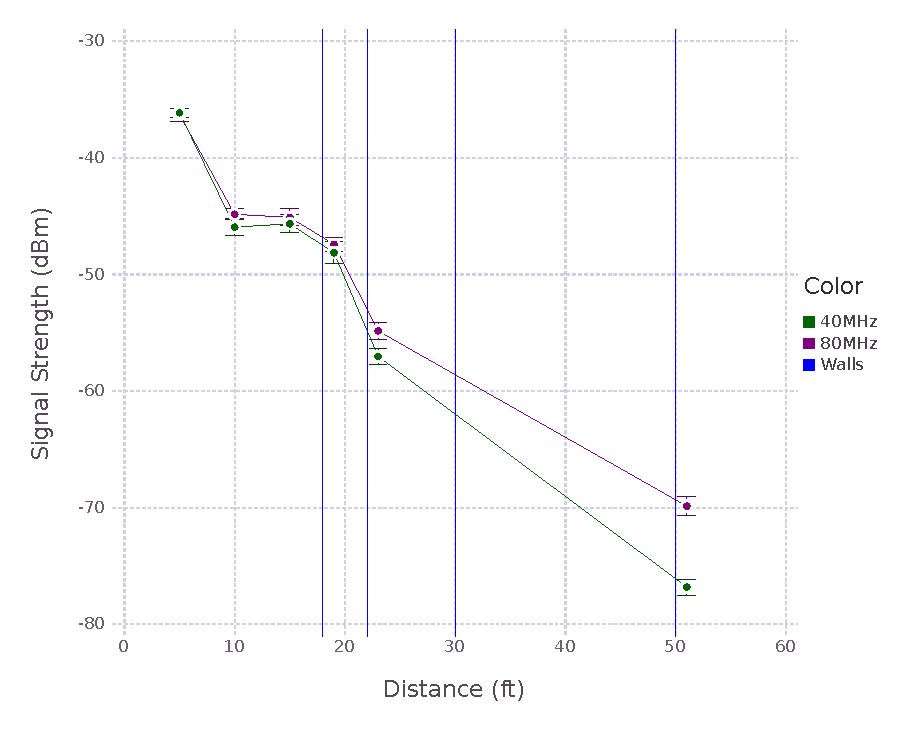
\includegraphics[width=0.5\textwidth]{figures/Intel_Inside_Beamformed}
\caption{Intel Indoor Signal}
\end{figure}

\section{Related Works}
%Related work, which discusses the current state of the art that you intend to build upon.
There is significant work on application level behaviors
\cite{verkaik2009softspeak}, environmental interferance
(\cite{kamerman1997microwave}, \cite{golmie2003interference},
\cite{shin2007mutual}, \cite{gummadi2007understanding}, etc), multiple
% Note check out gummadi2007understanding for ideas
crowded WAPs \cite{fuxjager2007myth} with 802.11b/g/n, and 802.11g/n
co-existing with other 2.4Ghz systems \cite{petrova2007interference}.

There is comparatively little real-world work with 802.11ac, as
clients and APs are only just becoming available. Current work
includes a single significant effort on real-world 802.11ac
performance indoors \cite{dianu2014measurement},the quite
comprehensive \cite{zeng2014first} and a large number of simulation
papers (\cite{bellalta2012performance}, \cite{ong2011ieee},
\cite{redieteab2012mu} , etc). The only real benchmarking is in
\cite{zeng2014first} and does include most of the topics we want to
explore. However, they don't fully explore the effects of a very
crowded 802.11b/g/n space on 802.11ac performance, or the effect of
802.11ac on b/g/n performance. The above two papers are the only
real-world tests we know of (these only just started appearing
mid-2014), and we are not aware of any significant work on 802.11ac
and b/g/n interactions with real-world testing in the academic
literature.

\section{Discussion}

The surface was seen to outperform the other systems in the indoor test at the furthest location. These results did not make any sense to us so we did some investigation into the packet captures. The Surface consistently sent at MCS indices 4 and 5 using two spatial streams for a theoretical data rate of 490 Mbps. The Intel card always sent at MCS index 2 with only 1 spatial stream for a theoretical data rate of 83 Mbps. This accounts for the difference in throughput between these two devices however the Mac was a special case. It used an MCS of 4 and 5 like the Surface but used 2 and 3 spatial streams consistently. However, the performance was hindered drastically by the amount of TCP retransmits that it received. Unfortunately we did not capture on the AP but we believe that the ACKs were not making it back to the AP when the Mac transmitted them. There were no retransmits at the 802.11 MAC layer so this indicated that the packet was resent by the other endpoint based on a timeout and the ACK packets sent by the Mac were unfortunately not captured to verify this behavior. The Mac also had performance issues when capturing its own packets and this appears to affect the throughput and timing such as turn around time for sending ACKs. One other peculiarity that both the Mac and Intel exhibited was the receive window size keep growing to a large value, where as on the Surface this value remained at 64K at all times. Once again, we did not capture packets at the other endpoint or AP so we were not able to resolve why this behavior was occurring exactly.

In the beginning we started to use iPerf version 3.0.11 but quickly discovered that it had some bugs/peculiar operations. When using iPerf3 for our testing we would always get higher throughput when the wireless client sent to the wired client. This was counter-intuitive to us, so we did some investigation and eventually tried iPerf 2 to see if this behavior was the same. It was not the same, it was as we expected, that the other direction (wired client to wireless client) was always a greater throughput.

We also started to use OpenWRT Chaos Calmer (Dev. branch) on the Linksys WAP so that we could have more flexibility, control, and insight into what the WAP was doing. However, after consistently experiencing poor performance of the WiFi network, we resorted back to the latest stock firmware to determine if the hardware or firmware was the cause. Once we had the stock firmware back in place, the performance of the WiFi network was as we expected. At this point, we stuck with the stock firmware and adjusted our testing framework to account for the lack of control at the AP where we could.

\section{Conclude}
Wireless measurement is difficult. Changing environmental factors and
lack of device introspection make drawing serious conclusions nearly
impossible with the current state of 802.11ac consumer products.

We have shown, however, that 80MHz channel widths perform
approximately as expected, increasing received signal strength both
indoors and outdoors, and increasing the maximum connection distance.
Unfortunately, most devices experience a net throughput reduction with
80MHz in the longest distance scenarios due to a combination of MCS
choice and a reduction (in the case of the Macbook and the Intel 7260)
to a single spatial stream under 80MHz.

We have learned that for future iterations of this project we need to increase the data set size.
This includes collecting frame captures at both end points and preferably on the AP as well. We also
have learned that more research needs to go into our equipment selection to better understand
the networking stack on each piece of equipment. We also need to select equipment that provides a symmetrical set of data, mainly all wireless equipment should be able to capture at full speed and provide full wiretap header information. Another factor to consider when we choose devices is the available storage capacity. We ran into collection issues on the Surface with hard drive storage space which limited our collection size.

We also learned that a considerable amount of time must be set aside for analyzing the data in order to extract information from the data set and to find patterns and trends.


{\small
\bibliographystyle{IEEEtranSN}
\bibliography{acreport}
}

\typeout{}

\end{document}
